\section{Оценка работы алгоритма для трёхмерной модели Изинга}

\subsection{Расчёт магнитных свойств}

Для первого набора симуляций трёхмерной модели Изинга была расмотрена область J = 0.5 - 0.63 и длины 100-300.

\begin{figure}[!h]
    \centering
    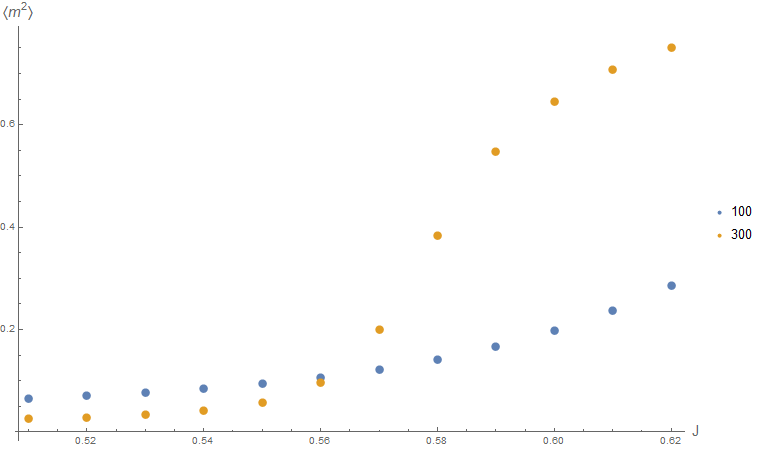
\includegraphics[width=100mm]{Sections/Images/m2_3D_50to60.png}
    \caption{График зависимости квадрата намагниченности от J}
    \label{fig:m2_3D}
\end{figure}

\begin{figure}[!h]
    \centering
    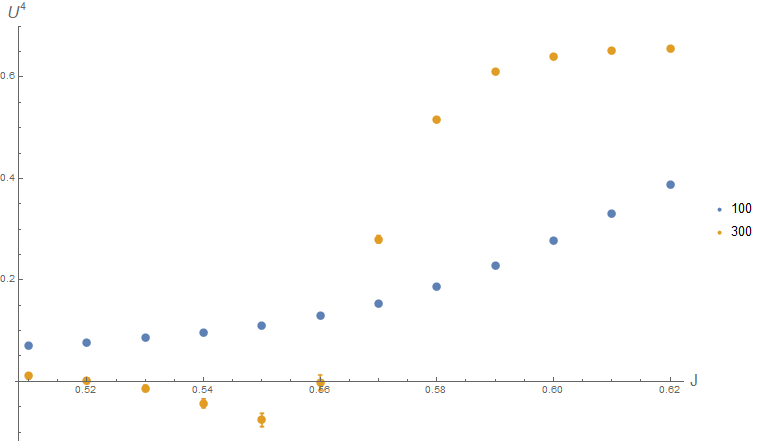
\includegraphics[width=100mm]{Sections/Images/U4_3D_50to60.png}
    \caption{График зависимости значения кумулянта Биндера от J}
    \label{fig:U4_3D}
\end{figure}

Полученные графики подтверждают первичные расчёты Камиллы, в том числе и неясную область отрицательных значений кумулянта Биндера.

\newpage